\documentclass[12pt]{article}
\usepackage{graphicx}
\usepackage{geometry}
\usepackage{fancyhdr}
\usepackage{titling}
\usepackage{amsmath}
\usepackage{amssymb}
\usepackage{enumitem}
\usepackage{xcolor}
\usepackage{circuitikz}
\usepackage{tikz}
\usepackage{subfigure}

\geometry{a4paper, margin=1in}

\title{\textbf{EE1200 - ELECTRIC CIRCUITS LAB}}
\author{EE24BTECH11012 - Bhavanisankar G S \\ EE24BTECH11019 - Dwarak A}
\date{\today}

\pretitle{%
    \begin{center}
    
\includegraphics[width=0.5\textwidth]{IITH.png}\\
    \vspace{1cm}
    \LARGE
}
\posttitle{\end{center}}

\begin{document}

\maketitle
\thispagestyle{empty}

\newpage

\section{TRANSIENT RESPONSE OF AN LC CIRCUIT}

\subsection{\textbf{AIM :}}
To study and analyze the transient response of an LC circuit, determine the natural frequency $\Omega_{n}$, and calculate the damping ratio $\zeta$ using theoretical and experimental methods.

\subsection{\textbf{APPARATUS REQUIRED: }}
\begin{itemize}
\item A 1 nF capacitor
\item A 2.2 mH inductor
\item DC power supply
\item An oscilloscope
\item Connecting wires
\item Probe
\end{itemize}

\subsection{\textbf{THEORY : }}
\begin{itemize}
\item An LC circuit consists of an inductor ( L ) and a capacitor ( C ) connected in parallel.
\item When a charged capacitor is connected to an inductor, energy oscillates between the capacitor's electric field and inductor's magnetic field.
\item But, in practicality, the components have their associated resistances, so the circuit essentially becomes an RLC circuit. Hence, the response eventually decays and becomes zero and becomes \textbf{damped oscillation} .
\end{itemize}

\subsection{\textbf{PROCEDURE : }}
\begin{itemize}
\item Connect the capacitor to a 5 V DC power supply. Once charged, disconnect it carefully without discharging it.
\item Connect the charged capacitor in parallel with the inductor. Ensure minimal resistance in the wiring.
\item The oscilloscope is used to monitor the voltage across the capacitor, and the natural oscillations are observed.
\item The natural frequency is calculated using theoretical method as given in the following section and the value is compared with the experimental value. 
\item The resistance across the inductor is found using a multimeter and the damping ratio $\zeta$ is estimated and compared with the observed value.
\end{itemize}

\subsection{\textbf{OBSERVATION : }}
\begin{itemize}
\item The waveform from the oscilloscope is recorded.
\item The oscillation period is measured using cursors.
\item The decay rate is measured.
\item From the graph, it can be seen that the damping frequency is approximately 90 kHz .
\end{itemize}

\subsection{\textbf{CALCULATION : }}
Consider the RLC circuit shown in Figure . The governing differential equation can be written as \\

\begin{figure}[!ht]
	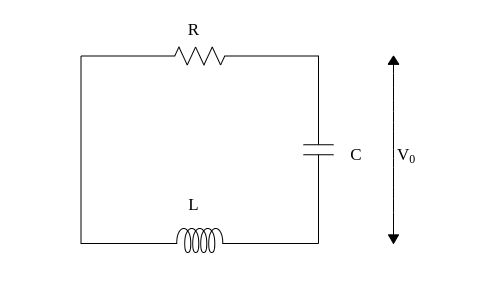
\includegraphics[width=\columnwidth]{circuit.png}
\end{figure}
\begin{align}
	\frac{d^2V}{dt^2} + \left(\frac{R}{L}\right) \frac{dV}{dt} + \frac{V}{LC} &= 0 \label{eq:de}
\end{align}
The damping coefficient, 
\begin{align}
	\zeta &= \frac{R}{2} \sqrt{\frac{C}{L}}
\end{align}
Considering $\zeta < 1$, we have, 
\begin{align}
	V &= V_{0} e^{\frac{-Rt}{L}} \left(cos(\Omega_{n} t ) + sin(\Omega_{n} t ) \right)
\end{align}
where, 
\begin{align}
	\Omega_{n} &= \frac{1}{\sqrt{LC}}
\end{align}
It can be seen that 
\begin{align}
	\Omega_{n} &= \frac{1}{\sqrt{2.2 \times 10^{-3} \times 10^{-9} }} \\
	&= 107 \text{ kHz} \\
	\zeta &= \sqrt{1 - (\Omega_{d}/\Omega_{n})^2} \\
	&\approx 0.55 \\
	R &\approx 1640 \Omega
\end{align}

\subsection{\textbf{CONCLUSION : }}
\begin{itemize}
\item It can be seen that the observed and calculated values are matching under the limits of experimental errors.
\item The dependence of $\Omega_{n}$ and $\zeta$ are established and explored. 
\end{itemize}

\begin{figure}[!htb]
\centering
\subfigure[Voltage across capacitor]{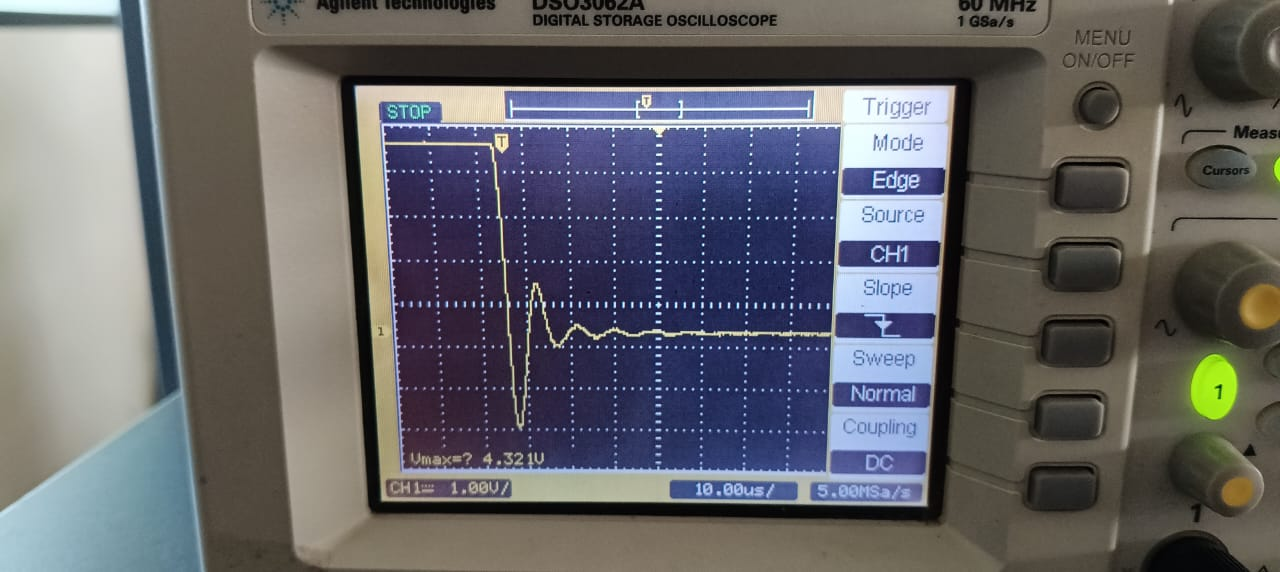
\includegraphics[width=0.45\textwidth]{fig_exp.jpg}}
\subfigure[Theoretical Result]{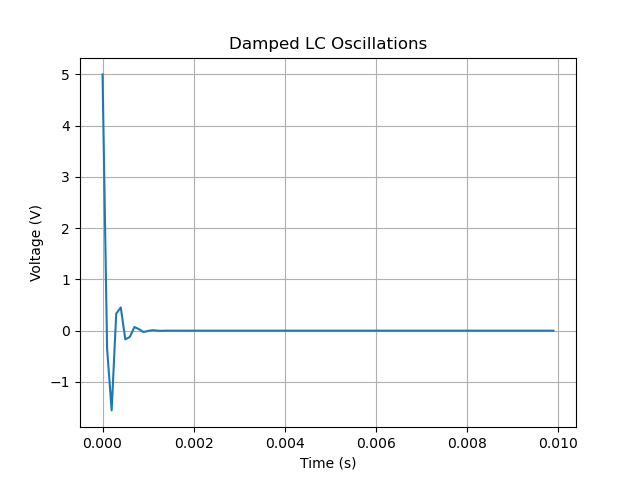
\includegraphics[width=0.45\textwidth]{codes/fig.png}}
\caption{Comparison of Experimental and Theoretical Results}

\end{figure}

\end{document}

